\section{The Advantage Of Traces}
\label{sec:advantage-traces}
In this section we present a qualitative evaluation of the witnesses and
traces that \toolname produces.

\begin{figure*}[ht]
\centering
\begin{minipage}{0.49\linewidth}
\centering
\begin{ecode}
let rec sqsum xs = match xs with
  | [] -> 0
  | h::t -> __(sqsum t)__ @ (h * h)
\end{ecode}
% File "sqsum.ml", line 3, characters 12-21:
\begin{verbatim}
Error: This expression has type
         int
       but an expression was expected of type
         'a list
\end{verbatim}
\end{minipage}
\begin{minipage}{0.49\linewidth}
\centering
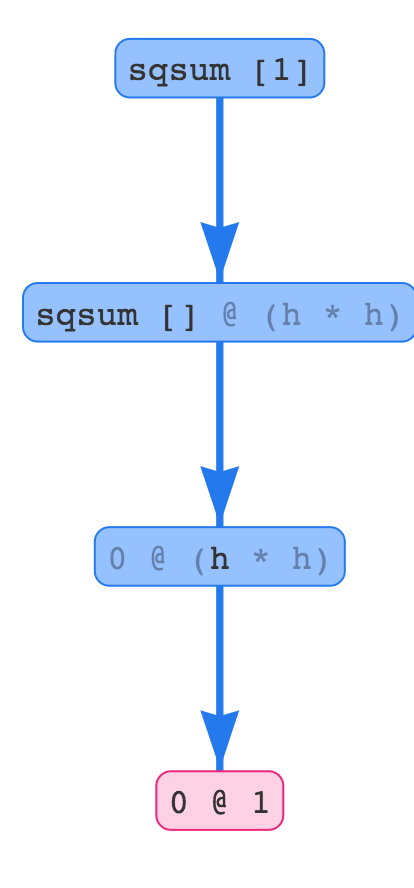
\includegraphics[height=125px]{sqsum.png}
\end{minipage}
\caption{caption}
\label{fig:traces}
\end{figure*}

\begin{figure*}[ht]
\centering
\begin{minipage}{0.49\linewidth}
\centering
\begin{ecode}
let rec sumList xs = match xs with
  | []    -> []
  | y::ys -> y + __sumList ys__
\end{ecode}
% File "sumList.ml", line 3, characters 17-27:
\begin{verbatim}
Error: This expression has type
         'a list
       but an expression was expected of type
         int
\end{verbatim}
\end{minipage}
\begin{minipage}{0.49\linewidth}
\centering
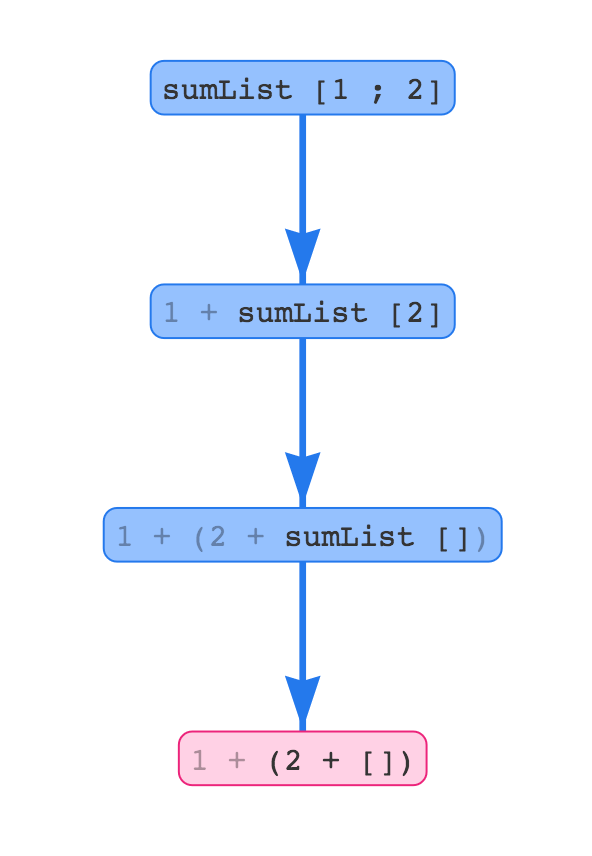
\includegraphics[height=125px]{sumlist.png}
\end{minipage}
\caption{caption}
\label{fig:traces}
\end{figure*}

\begin{figure*}[ht]
\centering
\begin{minipage}{0.49\linewidth}
\centering
\begin{ecode}
let append xs ys = match xs with
  | []   -> ys
  | h::t -> h :: __t__ :: ys
\end{ecode}
% File "append.ml", line 3, characters 17-18:
\begin{verbatim}
Error: This expression has type
         'a list
       but an expression was expected of type
         'a
       The type variable 'a occurs inside 'a list
\end{verbatim}
\end{minipage}
\begin{minipage}{0.49\linewidth}
\centering
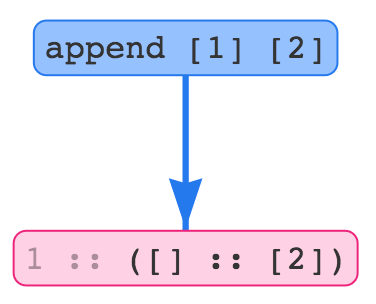
\includegraphics[height=75px]{append.png}
\end{minipage}
\caption{caption}
\label{fig:traces}
\end{figure*}

\begin{figure*}[ht]
\centering
\begin{minipage}{0.49\linewidth}
\centering
\begin{ecode}
let rec wwhile (f,b) =
  match f with
  | (z, false) -> z
  | (z, true)  -> wwhile (f, z)

let f x =
  let xx = x * x in
  (xx, (xx < 100))

let _ = wwhile (__f__, 2)
\end{ecode}
% File "wwhile.ml", line 10, characters 16-17:
\begin{verbatim}
Error: This expression has type
         int -> int * bool
       but an expression was expected of type
         'a * bool
\end{verbatim}
\end{minipage}
\begin{minipage}{0.49\linewidth}
\centering
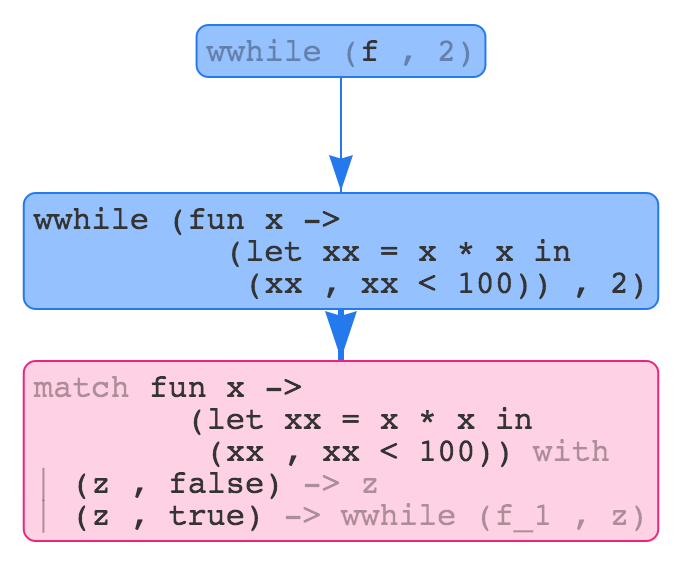
\includegraphics[height=150px]{wwhile.png}
\end{minipage}
\caption{caption}
\label{fig:traces}
\end{figure*}














%%% Local Variables:
%%% mode: latex
%%% TeX-master: "main"
%%% End:
